% !TEX program = pdflatex
% A4 paper, 11pt font, 2cm margins on all sides. Title page with two PDF logos.
% Table of contents starts on page 2, page numbering (arabic) starts at the TOC.
\documentclass[11pt,a4paper]{article}

% --- Encoding & Fonts (pdflatex) ---
\usepackage[utf8]{inputenc}
\usepackage[T1]{fontenc}
\usepackage{libertine} % Use Libertine font

% --- Page layout ---
\usepackage[a4paper,margin=2cm]{geometry} % 2cm margins on each side

% --- Graphics ---
\usepackage{graphicx} % for \includegraphics (supports .pdf logos with pdflatex/xelatex)

% --- Useful packages (optional) --- 
\usepackage{setspace}
\usepackage{hyperref}
\usepackage{amssymb}
\usepackage{amsmath}
\usepackage{subcaption}
\usepackage{algorithm}
\usepackage{algpseudocode}
\usepackage{multirow}
\usepackage[export]{adjustbox}
\usepackage{stmaryrd}
\usepackage{booktabs}
\usepackage[most]{tcolorbox}
\usepackage{colortbl}
\usepackage{xcolor}
\usepackage{wrapfig}
\usepackage[backend=bibtex,style=numeric]{biblatex}
\addbibresource{main.bib}
\hypersetup{colorlinks=true,linkcolor=black,urlcolor=blue,citecolor=black}

\tcbset{
  mybox/.style={
    colback=gray!10,   % background color
    colframe=gray!50,  % border color
    arc=3mm,           % rounded corners
    boxrule=0.5pt,
    left=2mm, right=2mm, top=1mm, bottom=1mm
  }
}

\tcbset{
  bluebox/.style={
    colback=blue!10,   % light blue background
    colframe=blue!50,  % border color
    arc=3mm,           % rounded corners
    boxrule=0.5pt,
    left=2mm, right=2mm, top=1mm, bottom=1mm
  }
}

\newcommand{\cm}{\checkmark}

% --- Section formatting ---
\usepackage{titlesec}
% Make all sectioning commands the same font size (Large) and bold
\titleformat{\section}{\Large\bfseries}{\thesection}{1em}{}
\titleformat{\subsection}{\Large\bfseries}{\thesubsection}{1em}{}
\titleformat{\subsubsection}{\Large\bfseries}{\thesubsubsection}{1em}{}

% Ensure consistent numbering depth and ToC
\setcounter{secnumdepth}{3}
\setcounter{tocdepth}{3}

% --- Metadata (fill these) ---
\newcommand{\ThesisTitle}{Data-Driven Estimation of Topological Features in 3D shapes}
\newcommand{\AuthorName}{Louis Martinez}
\newcommand{\AuthorAffiliation}{Télécom Paris}
\newcommand{\SupervisorName}{Maks Ovsjanikov}
\newcommand{\SupervisorAffiliation}{LIX, Ecole Polytechnique}
\newcommand{\MonthYear}{October 2025}

\renewenvironment{abstract}{
  \clearpage
  \begin{center}
    \Large\bfseries Abstract
  \end{center}
  \itshape
}{\par\clearpage}

\begin{document}

% ------------------
% Custom title page
% ------------------
\begin{titlepage}
    \centering
    \vspace*{2cm}

    {\LARGE\bfseries \ThesisTitle\par}
    \vspace{1.6cm}

    {\large \textbf{Author:} \\ \AuthorName \\[0.2cm]
    \AuthorAffiliation\par}

    \vspace{1.0cm}

    {\large \textbf{Supervisor:} \\ \SupervisorName \\[0.2cm]
    \SupervisorAffiliation\par}

    % --- Logos in the middle ---
    \vfill
    \begin{center}
        % Place your PDF logos in ./logos/ as logo1.pdf and logo2.pdf, or change the file names below
        \includegraphics[height=2.6cm]{logos/logo_mva.pdf}\hspace{1.2cm}%
        \includegraphics[height=2.6cm]{logos/logo_tp.pdf}
    \end{center}
    \vfill

    {\large \MonthYear\par}
\end{titlepage}

% ------------------
% Table of contents (starts on page 2)
% ------------------
\pagenumbering{arabic}
\setcounter{page}{1}
\tableofcontents
\clearpage

\begin{abstract}
\label{sec:abstract}
Large transformer-based foundation models have shown remarkable ability to extract expressive representations in a purely self-supervised, data-driven manner, and recent efforts have extended them to 3D shape understanding. In parallel, Topological Data Analysis (TDA), through the lens of persistent homology, offers mathematically grounded tools to characterize the structural information carried by point clouds. However, persistent homology scales poorly with dimension and sample size, limiting its applicability to large datasets. This thesis makes two main contributions. First, we investigate to what extent pretrained 3D transformer models capture structural, non-semantic properties of shapes, using TDA as a principled framework to quantify their topological awareness. Second, building on these insights, we introduce a data-driven proxy for persistent homology: a transformer-based approach that leverages learned representations to predict topological features efficiently. Our results highlight both the limitations of current 3D transformers and the potential of bridging foundation models with TDA to advance topology-aware 3D representation learning.
% Transformers have become the dominant architecture for representation learning across modalities, achieving strong performance in natural language processing and computer vision. This has motivated recent efforts to extend transformers to 3D shape understanding. While these models show promising results, they face two fundamental challenges. First, transformers are notoriously data-hungry, yet even the largest 3D shape datasets remain orders of magnitude smaller than those in text or vision. Second, although transformers perform well on simple benchmarks, they struggle with tasks that require reasoning about complex geometries and topologies. In particular, it is unclear whether pretrained 3D transformer models capture the structural, non-semantic properties of shapes, beyond surface-level geometric or categorical information. In this work, we systematically investigate this question. We demonstrate that current 3D transformers are intrinsically limited in their ability to capture such structural information, and we introduce a new procedure (tbd) that addresses this limitation and improves their capacity to represent challenging 3D shape properties.
\end{abstract}
\clearpage

% ------------------
% Main matter (each section in its own file)
% ------------------
\section{Introduction}
\label{sec:intro}


Foundation models for 3D data have emerged as a new paradigm for large-scale 3D shape understanding. Inspired by the success of self-supervised learning in natural language and vision, several transformer-based architectures have been adapted to 3D modalities such as point clouds, meshes, and voxels. These models learn expressive representations from unlabeled data and have achieved strong performance across tasks including classification, segmentation, and shape retrieval. The ability to extract rich, semantically meaningful features without manual supervision marks a significant step toward general-purpose 3D understanding.

Despite this progress, a key question remains open: \textit{What do 3D encoders learn about the structural properties of shapes?} While most studies have focused on evaluating semantic or geometric performance, little is known about whether these representations also capture deeper structural information such as topology. This limitation reflects a broader issue in the adaptation of self-supervised paradigms to 3D data. Pretraining strategies originally designed for text or 2D images have been directly transferred to 3D shapes, often without considering their unique mathematical and geometric properties. As a result, current models display restricted generalization. Encoders trained on object-centric datasets struggle to extend to large-scale scenes, whereas scene-level encoders often miss fine-grained shape details. Understanding the nature and limitations of these learned representations is therefore essential to assess whether these models truly capture intrinsic shape structure or simply memorize patterns present in their training distribution.

\subsection{Current State of Research}

Seminal work on self-supervised 3D encoders such as Point-BERT~\cite{pbert} and Point-MAE~\cite{pmae} have shown that transformer-based architectures can effectively model local and global geometric cues. They rely on masked modeling, or token reconstruction objectives to build shape embeddings. These embeddings have been empirically shown to correlate with geometric and semantic properties, yet they are rarely evaluated with respect to the topological structure of the underlying shape. Topology encodes the intrinsic organization of a shape beyond its local geometry. Capturing such information would indicate that a model understands the global connectivity and multi-scale structure of a 3D object, which is critical for robust generalization.

Topological Data Analysis (TDA) provides a mathematically principled framework for describing such structure. Through persistent homology, TDA quantifies the evolution of topological features such as connected components, loops, and voids as a scale parameter varies. These features form persistence diagrams, which summarize the underlying shape topology. TDA has been successfully used in physics, biology, and shape analysis~\cite{top_signatures} to measure structural complexity. However, it suffers from high computational cost: persistent homology scales poorly with both sample size and dimensionality, making it difficult to apply directly to modern 3D datasets with millions of points or high-resolution geometry.

Recent work has begun exploring connections between deep learning and TDA\cite{optimizing_persistent_homology, persistent_homology_seg, }. Neural networks can learn topological signatures~\cite{atol}, approximate persistence diagrams \cite{neural_approximation_graph_topological_features}, or embed topological features into latent spaces~\cite{topological_autoencoders}. Conversely, topological descriptors have been used to regularize or interpret neural representations~\cite{top_layer, topology_activations, top_reg}. However, few studies have investigated whether large pretrained 3D encoders implicitly learn topological information in their latent representations, and how this information compares to the explicit characterization provided by TDA.

\subsection{Motivations}

The goal of this report is to bridge the gap between representation learning and topological analysis for 3D shapes. There are three main motivations behind this work.

First, understanding how 3D shape encoders capture topology is fundamental to interpreting their learned representations. If these models encode persistent topological features, this would provide evidence that large-scale self-supervised training implicitly organizes representations around structural properties of shapes, not just visual or semantic correlations.

Second, topological data analysis offers a principled framework to quantify structural awareness. By comparing the topological signatures derived from a model’s latent space to those computed directly from geometry, we can evaluate whether the learned representations preserve key structural information. This enables a new kind of interpretability analysis grounded in topology.

Third, the connection can be turned the other way around. If 3D transformers already encode topological information, their representations could serve as efficient, data-driven proxies for topological computations. Since persistent homology is computationally expensive for large or high-dimensional datasets, learning-based approximations based on pretrained representations could scale topological reasoning to complex real-world 3D data.

The central problem investigated in this report can be summarized as follows:

\begin{center}
    \fbox{\parbox{0.9\linewidth}{
    \textit{To what extent do current 3D shape encoders capture the topological structure of 3D shapes, and can their learned representations be leveraged as scalable proxies for topological computations?}
    }}
\end{center}

Addressing this question contributes both to the interpretability of 3D foundation models and to the development of efficient topology-aware methods for large-scale geometric data.

\subsection{Contributions}

The contributions of this report are three-fold:

\begin{itemize}
    \item \textbf{A topology-controlled dataset.} We introduce DONUT (Section \ref{sec:topogen}), a scalable dataset of 3D shapes with full control over their topological properties. This dataset enables systematic evaluation of models’ sensitivity to structural variations.
    \item \textbf{A quantitative analysis of structural awareness.} We perform comprehensive experiments to measure how state-of-the-art unimodal 3D shape encoders capture structural, non-semantic information (Sections \ref{sec:used_models} and \ref{sec:ph}). Using persistent homology as an analytical tool, we assess the topological consistency of learned embeddings.
    \item \textbf{Architectural and training insights.} Based on the findings, we propose directions for improving 3D shape encoders, including architectural modifications and pretraining strategies that encourage topology-aware representations.
\end{itemize}
\section{DONUT: \underline{D}ataset \underline{O}f ma\underline{N}ifold str\underline{U}c\underline{T}ures}
\label{sec:topogen}

\begin{figure}[t]
  \centering
  \includegraphics[width=1.0\linewidth]{figs/topogen/samples_overview.png}

  \label{fig:topogen-samples}
  \caption{\textbf{Random samples from the dataset.} Despite the fact that each sample is generated from a rather small family of shapes, both the topology preserving placement and augmentations allow for a rich variety of shapes, while ensuring topological consistency.}
  \label{fig:short}
\end{figure}


Understanding how models capture topological properties of 3D shapes is a key step toward disentangling geometric representation learning from semantic categorization. Probing such capabilities requires datasets with explicit topological labels and fine-grained control over their distribution. However, existing 3D datasets, such as Objaverse~\cite{objaverse,objaverse_xl} or ShapeNet~\cite{shapenet}, focus primarily on semantic categories or low-level geometry, and do not provide systematic coverage of topological variation.

We introduce DONUT, a scalable dataset of synthetic 3D shapes annotated with accurate and balanced topological labels. Unlike prior datasets, DONUT is designed specifically to isolate intrinsic topological invariants, such as the number of connected components and the genus, enabling controlled evaluation of how models represent topology. This resource provides a foundation for probing, benchmarking, and training models on tasks where topological understanding is essential.

\subsection{Existing datasets}
\label{ssec:existing_datasets}

Existing 3D datasets provide only limited support for probing whether models capture topological structure. Broadly, they fall into three categories: combinatorial-only benchmarks, geometric datasets with noisy topology, and synthetic datasets with limited diversity.

\paragraph{Combinatorial benchmarks.}
The MANTRA dataset (Manifold Triangulation Assemblage) \cite{mantra} provides combinatorial triangulations of 2D and 3D manifolds, represented as abstract simplicial complexes without embedding in $\mathbb{R}^3$. MANTRA is a valuable testbed for assessing whether graph- or simplicial complex models capture higher-order structures such as Betti numbers $(\beta_0, \beta_1, \beta_2)$. However, since it lacks any geometric realization, MANTRA is not suitable for evaluating models built on geometric 3D representations such as meshes, point clouds, or implicit fields.

\begin{table}[h]
  \begin{center}
  \begin{tabular}{l l l l r}
  Dataset & \#Samples & \rotatebox[origin=lB]{90}{Meshes} & \rotatebox[origin=lB]{90}{Manifold} & \rotatebox[origin=lB]{90}{Balanced annot.}\\
  \midrule
  \rowcolor{green!20}
  \multicolumn{1}{l|}{DONUT}  & 30,000   & \cm & \cm & \cm \\
  \multicolumn{1}{l|}{MANTRA \cite{mantra}} & 43,100 & -- & \cm & -- \\
  \multicolumn{1}{l|}{ABC \cite{abc}} & 1,000,000+ & \cm & --   & -- \\
  \multicolumn{1}{l|}{Thingi10K \cite{thingi}} & 10,000 & \cm & -- & -- \\
  \rowcolor{green!20}
  \multicolumn{1}{l|}{EuLearn  \cite{eulearn}} & 3,300 & \cm & \cm & \cm \\
  \midrule
  \end{tabular}
  \end{center}
  \vspace{-2mm}
  \caption{\textbf{Overview of existing datasets and their capabilities.} We summarize here the main characteristics of existing datasets with topological annotations. Besides EuLearn, all existing datasets with topological annotations come with downsides, discussed in Section~\ref{ssec:existing_datasets}. However, since EuLearn seems to be the most promising dataset, we carried out an extensive analysis to (1) highlight limitations that make it unreliable for further experiments and (2) motivate the use of DONUT (see Appendix~\ref{ssec:suppl_eulearn_analysis}). \textit{Note:} The number of samples for MANTRA only takes into account 2-manifolds.}
  \label{tab:datasets}
\end{table}

\paragraph{Geometric datasets with noisy topology.}
Large mesh datasets such as Thingi10K~\cite{thingi}, Objaverse~\cite{objaverse} and ABC~\cite{abc} contain CAD models and artistic objects, and include coarse topological annotations (number of components, genus). However, these annotations are unreliable for several reasons:

\begin{enumerate}
  \item \textit{Discrepancy between raw and perceptual components.} Artistic and CAD models are typically constructed from many sub-meshes, so the annotated component count often diverges from the semantically meaningful object count.
  \item \textit{Severe class imbalance.} While a wide range of genus values is theoretically possible, the overwhelming majority of meshes in both datasets have genus 0–2, making them unsuitable for balanced probing tasks.
  \item \textit{Structural artifacts.} Many meshes are non-manifold or self-intersecting, rendering quantities such as the Euler characteristic ill-defined:
\begin{equation}
  \chi = V - E + F = 2 - 2g - b + c
  \label{eq:euler}
\end{equation}

where $V,E,F$ are the number of vertices, edges, and faces, $g$ is genus, $b$ the number of boundary components, and $c$ the number of connected components.
Attempts to repair such meshes (e.g., Manifold~\cite{manifold}, ManifoldPlus~\cite{manifoldplus}, DOGN~\cite{dogn}, CLAY~\cite{clay}) face tradeoffs between oversmoothing geometry, introducing artifacts, or incurring prohibitive computational cost. As a result, these datasets cannot provide reliable large-scale topological ground truth.
\end{enumerate}

\paragraph{Synthetic datasets with limited diversity.} 
The EuLearn dataset~\cite{eulearn} addresses class imbalance by generating surfaces of varying genus from Fourier curves. While balanced across genera, EuLearn suffers from two critical issues: (i) samples within each genus class lack diversity, making them nearly indistinguishable, and (ii) strong correlations emerge between genus and canonical orientation, enabling trivial classification via nearest-neighbor with Chamfer distance. Consequently, EuLearn fails to disentangle topological structure from geometric shortcuts, limiting its usefulness for robust probing.

\begin{figure}[h]
  \centering
  \includegraphics[width=0.5\linewidth]{figs/topogen/thingi_genus_hist.pdf}
   \caption{\textbf{Genus distribution of Thingi10K.} Both axes are plotted in log scale. The genus was estimated from the Euler characteristic, provided as metadata with the dataset; however, 2,651 samples do not fulfill the requirements to directly compute the genus from the Euler characteristic (see \ref{eq:euler}). They are therefore not taken into account here. The histogram shows that a large fraction of the dataset (over 3,000 samples out of 7,344) has genera of 0 or 1, indicating that higher-genus components are significantly underrepresented, which may limit accurate classification and probing analyses for those cases.}
   \label{fig:thingi-genus}
\end{figure}

\begin{figure}[h]
  \centering
  \includegraphics[width=0.5\linewidth]{figs/eulearn/dataset_samples.pdf}
   \caption{\textbf{Samples from the EuLearn dataset across different genera.} As the genus increases, shapes become geometrically more complex. This trend highlights a confounding factor in the dataset: geometric complexity grows together with genus. As a result, classification performance may be driven not only by topological information but also by correlated geometric cues.}
   \label{fig:eulearn-samples}
\end{figure}


\subsection{Method}
\label{ssec:topogen-method}

Since DONUT is made of synthetic shapes, two critical challenges must be addressed to ensure that the results obtained from this dataset are relevant. 1) Foundation models are pretrained on real shapes. Therefore, learned features reflect the distribution of real world geometry and semantics. Synthetic data, however, introduce patterns and biases that don't exist in real data, making them fall out-of-distribution. 2) Another common pitfall of synthetic datasets (cf. EuLearn) is the lack of variability, making evluation tasks such as probing, trivial. In practice, the first challenge is overcome by the fact that foundation models are pre-trained on datasets (e.g ShapeNet, Objaverse, etc.) that are large enough for synthetic shapes not to fall out-of-distribution. This is experimentaly validated in Figure (+ figure with umaps). To adress the second challenge, we developed a set of rules and augmentation techniques to ensure that the generated shapes are both diverse and topologically accurate.

Below we derive these rules used to generate DONUT, and more importantly, how the latter allow to maintain this variability across samples while scaling their number up to $10^5$ shapes.

\subsubsection{Labels Distribution}
\label{sssec:labels-distribution}

A central design choice in DONUT is to ensure balanced topological supervision across the dataset. To this end, both the genus and the number of connected components are sampled such that their marginal distributions are approximately uniform. This prevents any single topological class from dominating and guarantees that models trained on the dataset are exposed to the full spectrum of topological structures. We bring this guarantee over marginal distributions by first sampling the labels before actually generating any mesh. \ref{sec:topogen-complements} formally describes how the labels are sampled and further details the properties of the dataset we used for all our experiments

Each sample is further composed of multiple meshes selected from a predefined family of template shapes. This choice introduces large geometric variability while maintaining strict control over label balance. As a result, the dataset couples statistical uniformity in labels with broad diversity in shape realizations. Nevertheless, by limiting ourselves to certain families of geometric shapes, we avoided falling into the pitfall of geometric complexity mentioned earlier. 

\subsubsection{Sample-Level Properties}
\label{sssec:sample-level-properties}

At the level of individual samples, the generation process begins by selecting the global genus and number of connected components. These values are then distributed across the meshes composing the sample. For example, a sample may include one mesh of genus one, several genus-zero meshes, or even higher-genus meshes, depending on the chosen configuration.

Each mesh is then instantiated from a specific parametric family of shapes:
\begin{itemize}
  \item \textit{Genus 0:} Superellipsoids and cones
  \item \textit{Genus 1:} Supertoroids and cones
  \item \textit{Genus $\geq 2$:} K-tori
\end{itemize}

\textbf{Superquadrics.} Superellipsoids  (resp. toroids) are part of a wider family of parametric shapes called superquadrics. They were introduced by Barr et al. \cite{superquadrics} in 1981 and are widely used in computer graphics for their ability to represent a large range of shapes with a small number of compact parameters. Superquadrics have recently regained attention in 3D scene understanding, notably in SuperDec \cite{superdec}, because of their expressiveness and their ability to approximate complex structures by composition. Their implicit equation is given by:

\begin{equation}
\left( \left| \frac{x}{s_x} \right|^{\tfrac{2}{\epsilon_2}}
     + \left| \frac{y}{s_y} \right|^{\tfrac{2}{\epsilon_2}} \right)^{\tfrac{\epsilon_2}{\epsilon_1}}
+ \left| \frac{z}{s_z} \right|^{\tfrac{2}{\epsilon_1}}
= 1
\end{equation}

where $(s_x, s_y, s_z) > 0$ are scale factors along the $x, y, z$ axes respectively, and $(\epsilon_1, \epsilon_2) > 0$ are shape exponents that modulate the surface's roundness (resp. sharpness). Sampling these parameters within predefined ranges allows to efficiently sample a variety of shapes while maintaining control over their topological properties.

\subsubsection{Mesh Generation}
\label{sssec:mesh-generation}

One key challenge is to be able to generate a large amount of samples (up to $10^5$) in a reasonable amount of time. This order of magnitude is motivated the results of Point-MAE-Zero \cite{pmaezero}. Accurate representations were obtained with a pretraining set containing around 150K samples. While we further use DONUT essentially for evaluation/probing tasks, we want to preserve the possibility of scaling to pretraining regimes where data requirements are significantly higher. We therefore restrict as much as possible the use of computation intensive operations. k-tori aside, every mesh is generated either with its parametric expression when available, or with simple rules.

\paragraph{Cones.} \dots

\paragraph{Superquadrics.} Meshes corresponding to super ellipsoids and super toroids are generated directly from their parametric forms. The procedure consists of two steps: 1) generate a base template mesh (a sphere for ellipsoids, a torus for toroids) where vertices are expressed in spherical (resp. toroidal) coordinates, and 2) deform it according to the superquadric equations. This construction is lightweight, parallelizable, and supports fast large-scale dataset generation. The parametric equations we use in practice are as follows:
\begin{equation}
\begin{aligned}
\text{Ellipsoid} \quad
\begin{cases}
x(u,v) &= s_x \, C_{\epsilon_1}(v) \, C_{\epsilon_2}(u) \\
y(u,v) &= s_y \, S_{\epsilon_1}(v) \, S_{\epsilon_2}(u) \\
z(u,v) &= s_z \, S_{\epsilon_1}(v)
\end{cases}
\end{aligned}
\qquad
\begin{aligned}
\text{Toroid} \quad
\begin{cases}
x(u,v) &= s_x \, \bigl(R + C_{\epsilon_1}(v)\bigr) \, C_{\epsilon_2}(u) \\
y(u,v) &= s_y \, \bigl(R + S_{\epsilon_1}(v)\bigr) \, S_{\epsilon_2}(u) \\
z(u,v) &= s_z \, S_{\epsilon_1}(v)
\end{cases}
\end{aligned}
\end{equation}


where $u,v \in [-\pi, \pi]$ are the vertex coordinates of the template mesh is spherical (resp. toroidal) coordinates and:

\begin{equation}
\begin{aligned}
C_\epsilon(u) &= \operatorname{sign}(\cos(u)) \, |\cos(u)|^\epsilon \\
S_\epsilon(u) &= \operatorname{sign}(\sin(u)) \, |\sin(u)|^\epsilon
\end{aligned}
\end{equation}


\begin{figure}[t]
  \centering
  \begin{subfigure}[t]{0.48\linewidth}
    \centering
    \includegraphics[width=\linewidth]{figs/topogen/toroids_overview.png}
    \caption{Supertoroids.}
    \label{fig:toroids-overview}
  \end{subfigure}
  \hfill
  \begin{subfigure}[t]{0.48\linewidth}
    \centering
    \includegraphics[width=\linewidth]{figs/topogen/ellipsoids_overview.png}
    \caption{Superellipsoids.}
    \label{fig:ellipsoids-overview}
  \end{subfigure}
  \caption{Overview of different shapes obtained for fixed values of $a_i, i \in \{1, 2, 3\}$ and increasing values of $\epsilon_1$ (left to right) and $\epsilon_2$ (bottom to top). 
  (a) Different supertoroids. As mentioned in TO ADD, using these shapes for $k$-tori ($k \geq 2$) is challenging because they may not preserve the genus, for instance if some parts are too thin or sharp. 
  (b) Different superellipsoids.}
  \label{fig:overview}
\end{figure}

\paragraph{$K$-tori.} In the case of higher-genus meshes, there are no closed-form parametric equations. Instead, we leverage the implicit formulation of tori. A $k$-torus is generated by (1) evenly distributing tori on a circle, (2) blending their signed distance functions (SDF) through a smooth union operator, and finally (3) extracting the mesh via marching cubes with a grid-size. However, this process is more computationally intensive as it requires applying marching cubes the discretized SDF, whose complexity scales in $O(N^3)$ where $N$ is the grid size. And since we seek to have high quality meshes to preserve fine-grained details (here holes), we use a higher grid resolution.

To smoothly blend the SDF of each torus generated independently, we use the \textit{smooth minimum} operator:

\begin{equation}
\operatorname{softmin}_k(s_1, s_2, \dots, s_n) 
= -\frac{1}{k} \log \left( \sum_{i=1}^n e^{-k s_i} \right)
\end{equation}

Where $(s_1, s_2, \dots, s_n) \in \mathbb{R}^{(N^3)}$ are the SDF of individual tori and $k$ is a hyperparameter controlling the smoothness of the blending. This operator is applied voxel wise. In other words, each voxel of the blended SDF is assigned with the smooth minimum value of the individual SDF.

\subsubsection{Topological Consistency and Diversity}
\label{sssec:top-consistency}

We still have two challenges addressing. First, when placing components within a sample, we must ensure they don't overlap. At the same time, they need to be close enough to make the samples both topologically consistent and challenging enough for models to correctly identify the number of connected components. In early experiments, we observed that if components are too far apart, the task can be trivially solved using a simple KNN classifier with Chamfer distance. Second, even with careful placement, models tend to overfit, sometimes even when using simple linear heads on top of learned features, showing that this alone is insufficient to evaluate their true topological understanding. To increase variability while preserving topological labels, we apply transformations both at the sample level and the individual component level.

\paragraph{Consistency.} 
To address the first challenge, we developed a two-stage placement procedure. Suppose there are already some components correctly placed within a sample. To add a new component, we first place it randomly in the sample and then check for intersections with the existing components. Experimentally, we observed that a randomly placed mesh overlaps with at most two other components. If the new component overlaps with only one existing component, we identify the point on the new mesh that is most deeply inside the other component and push the new component along the opposite direction of the surface normal at that point. For intricate shapes, a single adjustment may create new overlaps, so we repeat this step five times. If overlaps remain after five attempts, the component is discarded and a new one is generated and randomly placed. This iterative procedure improves efficiency: in practice, one or two adjustments are sufficient to resolve overlaps, making it faster than discarding and regenerating components immediately.

\paragraph{Variability.} 
To further increase the diversity of DONUT while preserving topological labels, we apply transformations both at the sample level and at the component level. Commonly used rigid transformations, such as rotations and scaling, are applied to both components and full samples. At the component level, we do not apply translations to avoid creating overlaps that would break the overall topology of the sample. To introduce additional geometric variability, we also apply twisting deformations (Figure \ref{fig:twisted-comparison}). Without loss of generality, we assume that a component (or a full sample) lies within the unit sphere, as global scaling can be applied afterward. First, we uniformly sample a direction on the unit sphere, which defines an axis for the twist. Next, we define a smooth scalar function along this axis that determines the rotation angle. Finally, each vertex is rotated around the axis by the angle given by the scalar function evaluated at the point where the vertex projects along the axis. This procedure introduces non-rigid variability while preserving the genus and connectivity of each component and of the overall sample.

\begin{figure}[t]
  \centering
  \begin{subfigure}[t]{0.48\linewidth}
    \centering
    \includegraphics[width=\linewidth]{figs/topogen/ktori_overview.png}
    \caption{\textbf{Degrees of freedom allowed on $k$-tori.} 
    Prior to the sequence of transformations applied to each individual component (e.g. rotation, twisting) we allow some variability during the generation. 
    The x-axis represents the ratio \textit{major radius / minor radius}. 
    The y-axis shows how the template shape is modified as we increase the value of $k$ (i.e. the genus). 
    \textit{Note:} In the actual dataset, $1$-tori are generated with the parametric representation of supertoroids, since a regular torus is a particular case of supertoroid. 
    However, for $k \geq 2$, using a composition of $1$-tori is more reliable. 
    Some parameter sets can lead to undesirable holes in the final shape.}
    \label{fig:ktori-overview}
  \end{subfigure}
  \hfill
  \begin{subfigure}[t]{0.48\linewidth}
    \centering
    \includegraphics[width=\linewidth]{figs/topogen/twisted_comparison.png}
    \caption{\textbf{Effect of twisting.} 
    Original template shapes (left) are twisted along the purple axis (right). 
    Twisting deformations introduce non-rigid variability while preserving the genus and connectivity of each component. 
    Here the scalar function defined along the axis is affine between $-\pi/6$ and $\pi/3$. 
    We apply this augmentation at the component and sample level.}
    \label{fig:twisted-comparison}
  \end{subfigure}
\end{figure}

\subsection{Analysis}

This section provides a detailed characterization of DONUT. We first present dataset statistics, label distributions, and its relation to pretrained models. We then discuss baseline performance and introduce two complementary protocols designed to verify that models trained on DONUT actually capture topological features.

\subsubsection{General Properties}
\label{sssec:topogen-general-properties}

\paragraph{Dataset statistics.}
DONUT contains 29,517 samples divided into training, validation, and test splits of 80\%, 10\%, and 10\%. Each sample has between 1 and 6 connected components, with the total genus ranging from 0 to 10. A single component has genus at most 5 (corresponding to a 5-torus (Figure~\ref{fig:ktori-overview})). The dataset size was chosen to balance feasibility and reliability: smaller datasets led to overfitting while much larger datasets made experiments costly. Figure~\ref{fig:topogen-gen-comp-hist} reports the marginal distributions of genera and connected components.

\paragraph{Distributions and scalability.}
Figure~\ref{fig:topogen-umaps-overview} shows that synthetic samples from DONUT occupy the same representation space as training data used by common 3D encoders. This indicates that the dataset lies within the learned distribution of existing models rather than being out-of-distribution. In addition, Figure~\ref{fig:topogen-gen-time} reports the time required to generate different dataset sizes, showing that large-scale variants remain practical.

\subsubsection{Baselines and Transferability}
\label{sssec:topogen-transferability}

We trained several classical point-cloud models (PointNet, PointNet++, DGCNN) and recent persistence-based models (PersFormer, xPerT, PersLay) on DONUT. Results are reported in Table~\ref{tab:topogen-results}. Beyond in-distribution accuracy, a key question is whether these models actually capture topology or only rely on geometric characteristics.

Transferability provides a natural probe. To test this, we evaluated models on a curated subset of ABC. This set contains shapes whose geometry differs significantly from the training distribution, but whose topology is well characterized and within the label space. If models have learned topology, they should retain reasonable performance on ABC despite geometric differences. Table~\ref{tab:topogen-results} shows that DGCNN and specialized topological models maintain strong transfer, supporting the idea that DONUT encourages models to focus on topology. We note that weak transfer can also reflect limitations of current architectures rather than flaws in the dataset itself.

\begin{table}[h]
\centering
\begin{tabular}{l|ccc|ccc}
\toprule
 & \multicolumn{3}{c|}{\textbf{Genus}} & \multicolumn{3}{c}{\textbf{Connected Components}} \\
Model & MSE$\downarrow$ & Acc.$\uparrow$ & F1$\uparrow$ & MSE$\downarrow$ & Acc.$\uparrow$ & F1$\uparrow$ \\
\midrule
\multicolumn{1}{l}{} & \multicolumn{6}{c}{\textit{Point-based models}} \\
\midrule
PointNet~\cite{pointnet}   & -- & -- & -- & -- & -- & -- \\
PointNet++~\cite{pointnet++} &  -- & -- & -- & -- & -- & -- \\
DGCNN~\cite{dgcnn}      & 1.05/11.7 & 51.5/18.1 & 51.3/15.2 & 0.11/1.04 & 89.1/27.7 & 89.1/25.4 \\
\midrule
\multicolumn{1}{l}{} & \multicolumn{6}{c}{\textit{Persistence-based models}} \\
\midrule
PersFormer~\cite{persformer} & -- & -- & -- & -- & -- & -- \\
xPerT~\cite{xpert}      & -- & -- & -- & -- & -- & -- \\
PersLay~\cite{perslay}    & -- & -- & -- & -- & -- & -- \\
\bottomrule
\end{tabular}
\caption{\textbf{Performance of baseline models trained on DONUT and evaluated both in-distribution and on ABC.} Values are reported as \textit{DONUT/ABC}. We report mean squared error (MSE), balanced accuracy (Acc.), and balanced F1-score (F1). MSE is reported to capture how far off predictions are from the ground-truth on average, which is particularly relevant given the natural hierarchy of the labels (genus and connected components): misclassifying by a larger margin is more severe than a closer miss. }
\label{tab:topogen-results}
\end{table}


\subsubsection{Saliency Analysis}
\label{sssec:topogen-saliency}

To further understand model behavior, we visualize saliency maps on toy shapes. These maps highlight which regions contribute most to predictions. When trained to predict genus, models tend to focus on cycles, while for connected components they concentrate around contact points between shapes (Figure~\ref{fig:dgcnn-saliency}). Such results suggest that models attend to meaningful topological structures rather than exploiting geometric shortcuts.

\begin{figure*}[t!]
  \centering
  \includegraphics[width=\linewidth]{figs/topogen/umaps_overview.pdf}
  \caption{\textbf{UMAP embeddings of features learned by 3D encoders.} DONUT samples project into the same space as the original training data, indicating that they are not out-of-distribution.}
  \label{fig:topogen-umaps-overview}
\end{figure*}

\begin{figure}[t]
  \centering
  \begin{subfigure}[t]{0.66\linewidth}
    \centering
    \includegraphics[width=\linewidth]{figs/topogen/components_genus_hist.pdf}
    \caption{Label distributions for genus and connected components.}
    \label{fig:topogen-gen-comp-hist}
  \end{subfigure}%
  \hfill
  \begin{subfigure}[t]{0.33\linewidth}
    \centering
    \includegraphics[width=\linewidth]{figs/topogen/generation_time.pdf}
    \caption{Scalability of dataset generation.}
    \label{fig:topogen-gen-time}
  \end{subfigure}
  \caption{\textbf{General properties of DONUT.} \textit{(a),(b)} The marginal distributions of genus and connected components are approximately uniform, ensuring balanced supervision across topological classes. \textit{(c)} The time required to generate datasets of varying sizes demonstrates that even large-scale variants remain practical.}
  \label{fig:topogen-properties}
\end{figure}

% \begin{figure}[t]
%   \centering
%   \includegraphics[width=\linewidth]{figs/topogen/saliency_dgcnn.pdf}
%   \caption{Saliency maps for DGCNN. For genus prediction, saliency is concentrated around cycles. For connected components, saliency appears around contact points.}
%   \label{fig:dgcnn-saliency}
% \end{figure}


% \subsection{Analysis}

% \begin{figure*}[t!]
%   \centering
%   \includegraphics[width=\linewidth]{figs/topogen/umaps_overview.pdf}
%   \caption{\textbf{UMAP visualization of the feature space learned by the encoders.} To assess whether samples from DONUT fall within the representation space of models trained on large 3D datasets, we first extracted final features from the training set of each model and fit a two-dimensional UMAP embedding on these features. Both input and output sampling resolutions match the training configuration of each model. We then projected the features extracted from DONUT into this same embedding space. The resulting visualization shows that the synthetic samples occupy the same space as the original training data, indicating that the representations of DONUT occupy regions of the learned space rather than falling out-of-distribution. Interestingly, we observed that the structure of the UMAP fitted on ZeroVerse (composed only of synthetic samples) is extremely regular, and that DONUT representations are uniformly spread throughout the same range.}
%   \label{fig:topogen-umaps-overview}
% \end{figure*}

% \begin{table}
% \centering
% \begin{tabular}{l|ccc|ccc}
% \toprule
%  & \multicolumn{3}{c|}{\textbf{Genus}} & \multicolumn{3}{c}{\textbf{Connected Components}} \\
% Model & MSE$\downarrow$ & Acc.$\uparrow$ & F1$\uparrow$ & MSE$\downarrow$ & Acc.$\uparrow$ & F1$\uparrow$ \\
% \midrule
% PointNet~\cite{pointnet}   & -- & -- & -- & -- & -- & -- \\
% PointNet++~\cite{pointnet++} &  -- & -- & -- & -- & -- & -- \\
% DGCNN~\cite{dgcnn}      & 1.05/11.7 & 51.5/18.1 & 51.3/15.2 & 0.11/1.04 & 89.1/27.7 & 89.1/25.4 \\
% \midrule
% PersFormer~\cite{persformer} & -- & -- & -- & -- & -- & -- \\
% xPerT~\cite{xpert}      & -- & -- & -- & -- & -- & -- \\
% PersLay~\cite{perslay}    & -- & -- & -- & -- & -- & -- \\
% \bottomrule
% \end{tabular}
% \caption{\textbf{Classification accuracy of different models trained on TopoGen.} Values are reported as \textit{TopoGen/ABC}. All models have been trained on DONUT point-clouds with 4096 points. We then evaluated them on both the TopGen test set and on a curated subset of ABC. Since the latter contains imbalanced labels we only report top-k balanced accuracy (Equation~\ref{eq:balanced-accuracy}) with $k=1,2,3$ for genus and $k=1,2$ for the number of connected components.}
% \label{tab:topogen-results}
% \end{table}


% This section provides a detailed characterization of DONUT. We report the number of samples, examine the distribution of labels, and assess the relationship between the synthetic data and pretrained models used in our experiments. The goal is to establish a clear understanding of the dataset’s composition and ensure that it provides a meaningful and reliable basis for evaluation.

% \subsubsection{General Properties}
% \label{sssec:topogen-general-properties}

% \paragraph{Dataset statistics.} 
% All experiments (besides cross-validations) were conducted using the same training, validation, and test sets. DONUT contains 29517 samples in total, divided into splits of 80\%, 10\%, and 10\%, respectively. The dataset size was chosen as a trade-off: smaller datasets led to overfitting of the evaluated models, while larger datasets made even simple experiments computationally demanding. The goal was to construct a unified dataset that is both practical for experimentation and reliable for evaluation. Each sample contains between 1 and 6 connected components, with the total genus per sample ranging from 0 to 10. A single component has genus at most 5 (corresponding to a 5-torus). We also report the marginal distributions of the genus and the number of connected components (Figure~\ref{fig:topogen-gen-comp-hist}).

% \paragraph{Distributions and Scalability.} 
% Figure~\ref{fig:topogen-umaps-overview} highlights that DONUT lies within the distribution learned by the pretrained models we further evaluate.  To demonstrate the scalability  of the generation process, we also report the time taken to generate different versions of the dataset (Figure \ref{fig:topogen-gen-time}).

% \subsubsection{Transferability}
% \label{sssec:topogen-transferability}

% A central question in assessing models trained on our dataset is whether they truly capture topological information or merely exploit geometric shortcuts. Transferability provides a natural test: if a model encodes topology rather than incidental geometry, it should generalize to 3D shapes with the same topological labels but drawn from a distinct geometric distribution. To this end, we constructed a curated evaluation set from ABC, comprising several hundred shapes whose geometry lies outside the training distribution, yet whose topology is well-characterized and within the range of the label space. Successful performance on this set indicates that the learned representation is aligned with topology rather than geometry. A natural concern is that poor model performance might reflect limitations of current architectures rather than flaws in the dataset itself. Importantly, Table~\ref{tab:topogen-results} demonstrates that at both DGCNN and models tailored for topological features extraction demonstrate strong transferability. Training details for all models are provided in the Appendix~\ref{suppl:topogen-baseline-training}.




% \begin{figure}[t]
%   \centering
%   % First subfigure (2/3 width)
%   \begin{subfigure}[t]{0.66\linewidth}
%     \centering
%     \includegraphics[width=\linewidth]{figs/topogen/components_genus_hist.pdf}
%     \caption{\textbf{Labels distribution of TopoGen.} Samples are generated in such a way that the marginal distributions of genera and number of connected components are nearly uniform. More specifically, the number of components is exactly uniform by design (Algorithm~\ref{alg:topogen-labels-sampling}). However, one can show that the distribution of genera is a decreasing step function depending on both the maximum genus per component and the maximum genus per sample (see demonstration in Appendix). Even though this makes DONUT imbalanced for the genus label, effects on results are minimal since (i) the ratio between the most and least represented categories is close to 1, and (ii) DONUT contains enough samples for simple models to ``see'' the least represented categories enough times to make accurate predictions and not overfit on the training set. \textit{Note:} One can notice that the distribution of the number of components is not perfectly uniform, because some degenerate samples were discarded.}
%     \label{fig:topogen-gen-comp-hist}
%   \end{subfigure}%
%   \hfill
%   % Second subfigure (1/3 width)
%   \begin{subfigure}[t]{0.33\linewidth}
%     \centering
%     \includegraphics[width=\linewidth]{figs/topogen/generation_time.pdf}
%     \caption{\textbf{Generation time.} This log-log plot shows the time taken to generate different versions of DONUT with increasing number of samples. The generation is performed in parallel on 124 AMD Epyc CPU cores. Given all the constraints imposed on the samples and the high mesh quality, generating $6 \cdot 10^5$ samples is performed in a reasonable amount of time ($\sim 21$ hours). As a reference, the dataset used for \textit{Point-MAE-Zero}~\cite{pmaezero}, made of 150K samples, was generated in 600 CPU hours. For the same number of samples, the generation process used for DONUT would require $\sim 650$ CPU hours ($21 \,\text{hours} \times 124 \,\text{cores} \,/\, ((6.0 \cdot 10^5)/(1.5 \cdot 10^5))$). This further motivates the choice of using only $10^4$ samples for the experiments, as it takes around 2.5 hours to generate the dataset (dotted red lines).}
%     \label{fig:topogen-gen-time}
%   \end{subfigure}

%   \caption{General properties of DONUT.}
%   \label{fig:topogen-properties}
% \end{figure}






\subsection{Limitations and Further Improvements}

\paragraph{Topological Variety.} 
The current dataset has limited topological variety. It only encodes two characteristics: genus and number of connected components. This is mainly because all meshes are watertight and manifold. In this setting, topological invariants are trivial to deduce ($\beta_1= 2 \times \text("genus")$, $\beta_2=\beta_0$). A more challenging extension would include surfaces with boundaries, non-watertight meshes, or nested shapes. While the current generation process allows nested components in theory, no such cases are present in practice. Another direction is to incorporate families of parametric shapes with non-trivial topology, such as catenoids, helicoids, or Möbius strips.


\paragraph{Geometric Complexity.} The geometric diversity is also limited. It could be extended by adding parametric families that introduce richer geometric structures. For example, the Superformula introduced by Gielis (2003) \cite{superformula} generalizes superellipses and provides a broad range of shapes. Although we did not add such families here, since the dataset is mainly used for evaluation and no overfitting issues were observed with the current configuration, this would be valuable in other settings. In particular, if the dataset is used for pretraining, as in Point-MAE-Zero, introducing more geometric complexity would improve its utility.
\section{Used Models}
\label{sec:used_models}


This section provides an extensive description of the models used in our experiments. We focused on three main types of models: point cloud-based models, transformer-based models, and persistence-based models. Since the latter require background on persistence homology, they're further detailed in Section~\ref{ssec:ph}. On the one hand, point cloud-based models are used as baselines for specific tasks (see Table~\ref{tab:topogen-results}). This choice stems from the widely known limitations in terms of robustness to input corruption and generalization~\cite{set-transformer} of such models. On the other hand, transformers have demonstrated state-of-the-art performance on various 3D shape understanding tasks~\cite{pbert,pmae,pm2ae,pcpmae}, and we are therefore insterested here in their ability to learn rich representations from data.

\subsection{Baselines Models}
\label{ssec:baselines_models}

We compare results obtained with transformer-based models to several baselines widely used in the literature. These models directly act on individual points without any tokenization step. They are all invariant to point permutations and can handle varying point cloud sizes. A final feature vector is obtained through a global pooling operation, which is then used for downstream tasks.

\subsubsection{PointNet}

PointNet~\cite{pointnet} introduced the first deep learning architecture that operates directly on raw 3D points. Each point is independently transformed through shared multilayer perceptrons (MLPs) to extract per-point features, which are then aggregated using a symmetric pooling function—typically max pooling—to obtain a global shape descriptor. This design ensures invariance to input permutation and robustness to geometric transformations through a learned spatial transformer network. However, since PointNet treats each point independently before pooling, it lacks the ability to explicitly capture local geometric structures and neighborhood relations within the point cloud.

\subsubsection{PointNet++}

PointNet++~\cite{pointnet++} extends PointNet by introducing a hierarchical feature learning mechanism that captures local geometric patterns at multiple scales. It partitions the point cloud into overlapping local regions using sampling and grouping operations, applies PointNet within each region to extract local features, and recursively aggregates them to form higher-level representations. This hierarchical structure allows PointNet++ to model fine-grained local geometry while maintaining the permutation invariance of PointNet. The introduction of radius-based grouping and multi-scale feature extraction significantly improves robustness to non-uniform sampling and enhances generalization to complex shapes.

\subsubsection{DGCNN (Dynamic Graph CNN)}

DGCNN~\cite{dgcnn} further advances local structure modeling by representing the point cloud as a dynamic graph, where edges connect each point to its k-nearest neighbors in the feature space. Unlike PointNet++’s static grouping, DGCNN updates the neighborhood graph at each layer, allowing feature dependencies to evolve adaptively as the representation becomes more abstract. The model applies an edge convolution operator that learns features based on both point attributes and relative positional differences, effectively capturing local geometric relations and contextual information. This dynamic graph formulation enables DGCNN to achieve strong performance on tasks requiring fine spatial reasoning, such as segmentation and shape classification.

\subsection{Transformer-based models}
\label{ssec:transformer_based_models}

\begin{figure}[t]
  \centering
  \includegraphics[width=1.0\linewidth]{figs/transformer_overview.pdf}
   \caption{\textbf{Transformer Overview for 3D point-clouds.} A point cloud is first partitioned into local patches using farthest point sampling (FPS) and K nearest neighbors (KNN). Patches are then embedded and augmented with positional encodings. The resulting sequence of patch embeddings is processed by a Transformer encoder to produce a global shape representation.}
   \label{fig:transformer-overview}
\end{figure}

Recent advances in transformer architectures for 3D shape understanding have largely built on the intuition that ideas from NLP and vision can be transferred to point cloud data. While the geometry of 3D shapes is fundamentally different from text or images, most models share a similar pipeline. A point cloud is first partitioned into a set of local patches. This is commonly achieved with farthest point sampling, and then grouping each center with its nearest neighbors to form a subcloud. Each of these patches is then embedded into a high-dimensional space using a lightweight encoder, typically a variant of PointNet or DGCNN that aggregates local geometric features while maintaining permutation invariance.

To preserve spatial structure, positional encodings are added by projecting the coordinates of the patch centers through an MLP, which provides the transformer with a notion of relative geometry between patches. The resulting sequence of patch embeddings, optionally augmented with a learnable global "class token" is then fed into a Transformer encoder. This process is conceptually identical to Vision Transformers, where image patches are tokenized, embedded, and processed sequentially, though here the tokens correspond to irregular geometric neighborhoods rather than regular image patches.

This generic framework has provided the foundation for several influential works that differ primarily in how tokens are defined, how self-supervised pretraining is formulated, and whether hierarchical representations are incorporated. We now discuss these paradigms in detail.

\subsubsection{Point-BERT: Discrete Tokenization and Masked Modeling}
\label{sssec:pointbert}

One of the earliest attempts to port the BERT paradigm to point clouds is Point-BERT \cite{pbert}. Its central idea is to treat a point cloud as a sequence of discrete tokens, thereby enabling the use of masked language modeling (MLM) for self-supervised pretraining. To achieve this, Point-BERT first trains a discrete variational autoencoder (dVAE) to learn a vocabulary of geometric tokens. The encoder of the dVAE maps continuous patch embeddings into discrete codewords, while the decoder reconstructs the original patch from the codeword, ensuring that the learned vocabulary captures meaningful local geometry.

With this vocabulary in place, Point-BERT pretrains the Transformer using Masked Point Modeling (MPM): a subset of input patches are masked, and the model is trained to predict the corresponding discrete token indices assigned by the dVAE. This formulation parallels masked language modeling in NLP, where the model predicts missing words from context, but here the "words" are geometric patches. Importantly, Point-BERT also incorporates a learnable class token that is updated jointly with the patch tokens during pretraining. The final embedding of this class token is then used for downstream classification and retrieval tasks, mirroring the global semantics captured by the CLS token in NLP transformers.

This approach makes pretraining strongly analogous to BERT, but it requires a two-stage pipeline, first learning the tokenizer and then training the transformer, which introduces additional complexity. Nonetheless, Point-BERT demonstrated that masked token prediction is a powerful way to learn shape priors from unlabeled point clouds.

\subsubsection{Point-MAE: Continuous Tokens and Masked Autoencoding}

While Point-BERT relies on discrete tokenization, Point-MAE~\cite{pmae} instead follows the Masked Autoencoder (MAE)~\cite{mae} framework introduced in vision. Here, patches are represented by continuous embeddings rather than discrete vocabulary entries, and the pretraining task is reconstruction rather than classification. Specifically, Point-MAE applies a high masking ratio (often exceeding 60\%) to the input patches. Only the unmasked patches are fed through the heavy transformer encoder. Masked patches are replaced with a shared mask token, and both unmasked embeddings and mask tokens are processed by a lightweight decoder tasked with reconstructing the original 3D coordinates of the masked patches.

This approach has several advantages. First, it avoids the need for a separate tokenizer, simplifying the training pipeline. Second, it is more computationally efficient: since the encoder processes only unmasked patches, the model scales better to large point clouds. Third, it allows the model to directly learn continuous geometric representations, which are more flexible than a finite vocabulary.

Unlike Point-BERT, Point-MAE does not include a CLS token during pretraining. Instead, the class token is introduced only when the model is fine-tuned on downstream tasks. This choice emphasizes that the focus of pretraining is purely local reconstruction, while global semantics can be learned in task-specific adaptation. Overall, Point-MAE demonstrated that masked autoencoding provides a simple yet effective way to pretrain 3D transformers, establishing a new standard for self-supervised learning on point clouds.

\subsubsection{Hierarchical Extensions: Multi-Scale Representations}
\label{sssec:hierarchical_extensions}

A third line of work emphasizes that 3D shapes are inherently hierarchical, with geometric structures manifesting at multiple scales. This insight parallels the evolution from PointNet to PointNet++, where hierarchical feature extraction proved essential for robust representation learning. 

Point-M2AE~\cite{pm2ae} extends Point-MAE by introducing a multi-scale transformer architecture. The encoder progressively downsamples the point cloud into coarser patches, capturing increasingly global features, while the decoder reconstructs masked patches using skip connections, reminiscent of U-Net architectures. In addition, Point-M2AE employs a multi-scale masking strategy to ensure consistency across levels of abstraction and introduces local spatial self-attention at fine scales to better capture detailed geometry. This design not only improves parameter efficiency but also strengthens the model’s ability to capture structures across varying spatial resolutions.

\subsubsection{Further Improvements}
\label{sssec:further_improvements}

Most recent approaches have mainly built on top of Point-MAE, primarily for the training setting, easier than Point-BERT. PCP-MAE~\cite{pcpmae} modifies positional encoding to prevent information leakage: instead of directly using patch centers, which can trivially reveal masked locations, it requires the model to predict them. HFBRI-MAE~\cite{hfbrimae} incorporates handcrafted rotation-invariant features as both tokens and positional encodings, improving robustness under arbitrary 3D rotations. Point-RAE~\cite{prae} proposes a regression-before-autoencoding strategy to decouple encoder and decoder representations, thereby avoiding the risk of the decoder dominating feature learning. Collectively, these hierarchical and refined models show that injecting geometric inductive biases into the transformer architecture can significantly improve generalization and robustness.

\subsubsection{Comparative View}
\label{sssec:comparative_view}

Despite their differences, Point-BERT, Point-MAE, and their hierarchical successors share a common foundation: the adaptation of the transformer paradigm from language and vision to point clouds through \textit{patchification}, embedding, and positional encoding. What distinguishes them is how tokens are defined, how the self-supervised objective is formulated, and whether hierarchical geometry is explicitly modeled. Discrete-token approaches like Point-BERT require a two-stage pretraining pipeline but tightly align with NLP pretraining paradigms. Continuous-token methods like Point-MAE are simpler and more efficient, emphasizing reconstruction over classification. Hierarchical extensions such as Point-M2AE incorporate multiscale representations, bringing additional inductive structure into the transformer.

An important consequence of these differences is that evaluation protocols vary across models. Point-BERT pretraining relies on predicting discrete token IDs, while Point-MAE and M2AE use reconstruction losses such as Chamfer distance. The role of the CLS token also differs, being central during pretraining in Point-BERT but absent in MAE-style approaches. As a result, downstream fine-tuning and linear probing must be carefully adapted to each architecture. The precise evaluation settings for each method will be detailed in the following experimental section.
\section{Experiments}
\label{sec:experiments}

This section presents a series of experiments designed to investigate the relationship between learned 3D representations and topology. Our goal is to understand whether and how transformer models capture topological features of shapes, when trained on standard 3D data. We progressively move from a direct evaluation of encoded topology to more indirect analyses. Throughout these experiments, we use DONUT as the main benchmark.

We first conduct a probing analysis to estimate how much topological information can be linearly decoded from the representations of different layers (Section~\ref{ssec:model_probing}). This experiment provides an initial view of the presence and organization of topological cues inside the network. We then study the alignment between the learned embedding space and topological structures derived from persistent homology (Section~\ref{ssec:ph}). This second analysis gives a more geometric perspective on how representations relate to the shape topology. Finally (Section~\ref{ssec:changing_pretraining_data_distribution}), we investigate how changing the pretraining data distribution affects these findings, showing that current pretraining corpora do not explicitly encourage the capture of topological structures.

\subsection{Model Probing}
\label{ssec:model_probing}

\begin{figure}[h]
  \centering
  \includegraphics[width=\linewidth]{figs/probing.pdf}
  \caption{\textbf{Linear probing accuracy across transformer layers for Point-BERT (left column) and Point-MAE (right column).} We report probing accuracy for connected components (top row) and genus (bottom row). For each setting, accuracy values are averaged over the validation sets from a 5-fold cross-validation procedure, with error bars representing the corresponding standard deviations. For Point-BERT, probing is applied to the CLS token, which aggregates global information throughout the network. For Point-MAE, which does not include a CLS token during pretraining, we instead use the max-pooled patch embeddings from each layer.}
  \label{fig:probing-results}
\end{figure}

We start by probing transformer models to assess whether their internal representations encode information about shape topology. Specifically, we test if simple linear classifiers can recover the genus and number of connected components of shapes from the DONUT dataset using the representations of each intermediate layer. This approach provides a first estimate of how topological signals are distributed across the model depth.

\paragraph{Motivation.}
Linear probing is a standard approach in representation learning to evaluate how much a given factor of variation is linearly accessible from the learned embeddings. It assumes that if a linear classifier performs well, the corresponding information is already represented in a linearly separable manner. Importantly, several works have shown that the most informative representations for downstream tasks are not always located in the final layers of a model. Intermediate layers can encode more general or transferable structures before they are transformed into task-specific representations. This has been established in both vision and language transformers~\cite{intermediate_layers, structural_probe, vit_probing}. We therefore analyze not only the final layer, but the entire depth of each model, to capture where topology-related features emerge.

\paragraph{Experimental setup.}
For each evaluated model, we freeze the pretrained backbone and extract offline activations from all transformer layers on the DONUT dataset. At every layer $l$, we train two separate linear classifiers on top of the frozen representations to predict (i) the genus and (ii) the number of connected components. We perform 5-fold cross-validation and report averaged accuracy on the validation set.

\paragraph{Results.}
Overall, Figure~\ref{fig:probing-results} probing accuracy tends to increase with network depth for both models, indicating that higher transformer layers capture richer structural information. The improvement is modest for genus prediction, with an average increase of about 3\% between the first and last layers. In contrast, connected component prediction improves by roughly 8\%, suggesting that the notion of component separation becomes more explicit as features become increasingly global. This aligns with the expectation that transformers progressively aggregate local patch information into holistic shape-level representations.

Interestingly, in Point-MAE, accuracy for genus prediction plateaus after layer 5. This saturation may reflect the limited capacity of shallow hierarchies to encode topological invariants that depend on multi-scale relationships between local patches. Testing deeper or hierarchical variants of Point-MAE could help determine whether such information emerges later in the network.

Despite these relative improvements, absolute scores remain low: around 20\% for genus and 50\% for connected components, highlighting that both models only weakly encode topology. This supports the view that current pretraining objectives, which focus on geometric reconstruction or semantic alignment, do not drive models to capture global connectivity. While deeper layers improve aggregation and invariance, they remain sensitive to geometric details rather than structural invariants. These results reinforce that topology-aware objectives or explicit topological supervision may be required to make 3D encoders truly aware of shape structure beyond geometry.

\subsection{Subspace Alignment with Persistent Homology}
\label{ssec:ph}

\begin{figure}[h]
  \centering
  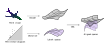
\includegraphics[width=\linewidth]{figs/alignment.pdf}
  \caption{\textbf{Alignment procedure overview.} We extract features from a 3D point cloud with the model we seek to evaluate. We also vectorize its corresponding persistence diagram (Section~\ref{sssec:vectorization_persistence_diagrams}). We then compute the CKA similarity (Section~\ref{sssec:subspace_alignment_protocol}) between the two sets of features to quantify how well the learned representation aligns with topological signatures.}
  \label{fig:alignment}
\end{figure}

We study the relationship between representations learned by 3D shape encoders and those derived from persistent homology. Following the perspective of the Platonic Representation Hypothesis~\cite{plato,platonic}, we view learned embeddings as potentially containing subspaces that capture intrinsic structural information. Information captured by persistent homology can also be treated as a complementary modality. Assuming there's a way to encode topological features into a vector space, we can then ask whether the learned and topological subspaces align. It's worth noticing that the analogy with \cite{platonic} is not perfect: while it's assumed that representations tend to converge at scale, topological features, even learned ones, aren't the result of large scale training.

We first review background on persistent homology and its vectorization. We then formally define the metrics used to quantify alignment. Finally, we describe our alignment protocol and present results across encoders and datasets.


\subsubsection{Persistence Diagrams}
\label{sssec:persistence_diagrams}


\paragraph{Filtrations.}
Let $(X, \leq)$ be a topological space equipped with a real index. A (real) filtration is a family of subspaces $(X_a)_{a\in\mathbb{R}}$ with $X_a \subseteq X_b$ whenever $a \leq b$ and $\bigcup_a X_a = X$. Typical examples are sublevel sets of a function $f:X\to\mathbb{R}$, namely $X_a = f^{-1}((-\infty,a])$.

\paragraph{Homology and persistent maps.}
Fix a field $\Bbbk$ and compute singular or simplicial homology with coefficients in $\Bbbk$. For $k\ge 0$ and $a\le b$, the inclusion $X_a \hookrightarrow X_b$ induces a linear map
\begin{equation}
i_{a}^{b}: H_k(X_a;\Bbbk) \longrightarrow H_k(X_b;\Bbbk).
\end{equation}
A $k$-dimensional class $\alpha\in H_k(X_b)$ is \emph{born} at the smallest $a$ for which it has a representative in $H_k(X_a)$, and it \emph{dies} at the smallest $d>b$ where it maps to zero in $H_k(X_d)$ under $i_{b}^{d}$. Classes that never die are called \emph{essential}.

\paragraph{Persistence modules, barcodes and diagrams.}
The collection $\{H_k(X_a), i_{a}^{b}\}_{a\le b}$ is a persistence module. Under standard finiteness conditions (e.g. $f$ tame, or finite type filtrations), it decomposes into interval modules. This gives a multiset of intervals (the barcode) or equivalently a multiset of points $(b_i,d_i)$ in the open half plane $\{(x,y)\in\mathbb{R}^2: x<y\}$ together with the diagonal $\{(t,t)\}$ available for matching with infinite multiplicity. This multiset is the $k$-th persistence diagram $\mathrm{Dgm}_k(X)$.

\paragraph{Why a persistence diagram is not a Euclidean vector object.}
A persistence diagram is a collection of points in the plane, where each point $(b,d)$ records the birth and death of a topological feature during a filtration. Points on the diagonal $(b=d)$ correspond to features that disappear immediately, and we assume there are infinitely many of them so that every feature in one diagram can be matched to a trivial one in another when comparing diagrams. Unlike vectors in Euclidean space, persistence diagrams cannot be naturally added or scaled, since such operations would destroy their topological meaning. Even computing an average of several diagrams can give multiple different results. In some cases, a diagram may even have infinitely many points away from the diagonal if the underlying space behaves badly. Therefore, persistence diagrams are treated as elements of a metric space, with distances defined by measures such as the bottleneck or Wasserstein metric, rather than as vectors in a linear space.

\paragraph{Distances between diagrams.}
Let $D$ and $E$ be diagrams. We allow matchings to the diagonal. The \emph{bottleneck distance} is
\begin{equation}
d_B(D,E) \;=\; \inf_{\gamma:D\to E} \; \sup_{x\in D} \, \lVert x - \gamma(x) \rVert_{\infty}.
\end{equation}
For $1\le p<\infty$, the $p$-\emph{Wasserstein distance} is
\begin{equation}
d_{W,p}(D,E) \;=\; \left( \inf_{\gamma:D\to E} \; \sum_{x\in D} \lVert x - \gamma(x) \rVert_{\infty}^{\,p} \right)^{1/p}.
\end{equation}
These are the standard and stable distances on persistence diagrams. The plain Hausdorff distance between the underlying point sets does not account for multiplicities and diagonal matchings and is not used in modern stability theory.

\paragraph{Stability theorems.}
For sublevel set filtrations of functions $f,g:X\to\mathbb{R}$ on a common triangulable space, the diagrams are stable under perturbations of $f$:
\begin{equation}
d_B\big(\mathrm{Dgm}_k(f), \mathrm{Dgm}_k(g)\big) \;\le\; \lVert f-g \rVert_{\infty}.
\end{equation}
Related bounds hold for $d_{W,p}$. In the algebraic language of persistence modules, the Isometry Theorem states that for $q$-tame modules $M,N$,
\begin{equation}
d_B\big(\mathrm{Dgm}(M), \mathrm{Dgm}(N)\big) \;=\; d_I(M,N),
\end{equation}
where $d_I$ is the interleaving distance.


\begin{figure}[t]
  \centering
  % Top full-width subfigure
  \begin{subfigure}{\linewidth}
    \centering
    \includegraphics[width=\linewidth]{figs/ph/expers_v2.pdf}
    \caption{Sub- (resp. super-) level set filtration.}
    \label{fig:filtrations_top}
  \end{subfigure}

  \vspace{0.5em} % space between top and bottom row

  % Bottom two subfigures
  \begin{subfigure}{0.48\linewidth}
    \centering
    \includegraphics[width=\linewidth]{figs/ph/expers2_ord_v2.pdf}
    \caption{Ordinary persistence diagram.}
    \label{fig:filtrations_left}
  \end{subfigure}\hfill
  \begin{subfigure}{0.48\linewidth}
    \centering
    \includegraphics[width=\linewidth]{figs/ph/expers2_v2.pdf}
    \caption{Extended persistence diagram.}
    \label{fig:filtrations_right}
  \end{subfigure}

  \caption{\textbf{Ordinary vs extended persistence.} (Figures adapted from \cite{perslay}). In \ref{fig:filtrations_top}, each node of the graph is assigned its height. Persistence intervals are shown under the sequence. In \ref{fig:filtrations_left}, ordinary persistence captures connected components and loops, but essential classes lead to infinite intervals (black and green markers) and the upward branch (blue) isn't captured. In \ref{fig:filtrations_right}, extended persistence pairs all classes at finite values by combining sublevel and superlevel filtrations with relative homology. Finally, $\text{Ext}_0^+$, $\text{Ext}_1^-$, $\text{Ord}_0$ and $\text{Ord}_1$ denote the different types of pairs in extended persistence.}
  \label{fig:filtrations}
\end{figure}


\paragraph{Extended persistence.}
Essential classes can lead to pairs with infinite lifetime. Extended persistence remedies this by combining sublevel and superlevel filtrations and using relative homology. For a function $f:X\to\mathbb{R}$ on a compact space, consider the sublevel filtration $(X_a)$ and the superlevel filtration $(X^a = f^{-1}([a,\infty)))$. One constructs a zigzag that passes from absolute to relative homology so that every class is paired at a finite parameter value. The resulting \emph{extended persistence diagram} has only finite pairs and encodes essential features as finite points. Figure~\ref{fig:filtrations} illustrates the filtration process as well as the difference between ordinary and extended persistence on a simple graph.


\subsubsection{Vectorization of Persistence Diagrams}
\label{sssec:vectorization_persistence_diagrams}

\begin{figure}[t]
    \centering
    \begin{subfigure}[b]{0.23\textwidth}
        \includegraphics[width=\textwidth]{figs/ph/examples/pd_example.pdf}
        \caption{Persistence Diagram}
    \end{subfigure}\hfill
    \begin{subfigure}[b]{0.23\textwidth}
        \includegraphics[width=\textwidth]{figs/ph/examples/landscape_example.pdf}
        \caption{Persistence Landscape}
    \end{subfigure}\hfill
    \begin{subfigure}[b]{0.23\textwidth}
        \includegraphics[width=\textwidth]{figs/ph/examples/persistence_image_example.pdf}
        \caption{Persistence Image}
    \end{subfigure}\hfill
    \begin{subfigure}[b]{0.23\textwidth}
        \includegraphics[width=\textwidth]{figs/ph/examples/betti_curve_example.pdf}
        \caption{Betti Curve}
    \end{subfigure}
    \caption{\textbf{Common prescribed vectorizations of a persistence diagram.} From left to right: (a) A sample persistence diagram with points representing topological features; (b) Persistence landscape capturing the prominence of features across scales; (c) Persistence image providing a smoothed, grid-based representation; \textit{Note:} Instead of considering persistence pairs as a \textit{(birth,death)} tuple, persistence image is fitted on $(birth, death-birth)$ pairs. (d) Betti curve showing the count of features over filtration values.}
    \label{fig:ph-vectorizations}
\end{figure}

Vectorizing persistence diagrams is crucial for incorporating topological signals in standard learning pipelines. A persistence diagram is a multiset of points in the plane. It does not live in a vector space and is usually compared with bottleneck or Wasserstein distances rather than inner products. Most learning algorithms expect fixed size vectors or a Hilbert space structure, so raw diagrams are not a natural input. Diagrams also have variable size and are permutation invariant, which complicates batching and optimization. These issues motivate stable feature maps and kernels that embed diagrams into Euclidean 

\textbf{Prescribed Vectorization.} Handcrafted summaries (Figure~\ref{fig:ph-vectorizations}) have long been the dominant strategy for vectorizing persistence diagrams in machine learning. The most common approaches include persistence landscapes \cite{persistence_landscapes}, Betti curves \cite{betti_curves}, and persistence images \cite{persistence_images} (Figure~\ref{fig:ph-vectorizations}). Landscapes embed diagrams in a Hilbert space and enable classical statistics, but they still require design choices such as the number of landscape levels and sampling resolution. Betti curves collapse a diagram to simple counting functions over the filtration. Persistence images rasterize diagrams with a kernel on a fixed grid. These methods are stable in theory but depend on key hyperparameters such as grid resolution and kernel width. These choices must be tuned per task and can limit expressiveness and generalization. Finally, ATOL \cite{atol} proposes an unsupervised alternative. It vectorizes measures, including sets of persistence points, by first clustering with K-means and then summarizing cluster statistics in a fixed length descriptor. The pipeline is simple and fast but remains sensitive to the chosen number of clusters and to the distribution shift between training and test diagrams.

\textbf{Learned Vectorization.} Recent work has moved from handcrafted features to learning based approaches \cite{adaptive_topological_feature},\cite{topological_signature} that act on persistence diagrams more directly, often through extended persistence \cite{extended_persistence} (see Section ...). PersLay \cite{perslay} introduces a neural layer that learns stable weights and pooling functions over points in a diagram. It was developed for graph tasks and relies on extended persistence to encode informative signatures before the learned aggregation. PLLay \cite{pllay} follows a hybrid route. It first computes persistence landscapes and then applies a differentiable neural layer that learns how to weight and combine landscape coordinates. This reduces manual feature design while keeping the stability benefits of landscapes. Transformer based designs have also appeared. Persformer \cite{persformer} treats each persistence point as a token and applies standard self attention. This is flexible but scales poorly as the number of points grows. To address scalability, the Multiset Transformer \cite{multiset_transformer} clusters points and modifies attention to account for multiplicities, so that a cluster can be handled as a single item with weight greater than one. This change reduces memory and time while preserving permutation invariance at the multiset level. xPerT \cite{xpert} goes further by leveraging sparsity with a \textit{pixelized diagram} representation. It is close in spirit to persistence images but does not require a smoothing kernel. The pixeliaation allows efficient tokenization and improves scalability compared with Persformer. xPerT also works with extended persistence; details are deferred to the dedicated section.

Across these learning based methods, a common trait is that the diagram is manipulated explicitly rather than replaced by coarse handcrafted summaries. Most results to date are on graph benchmarks rather than 3D shape understanding. This gap limits conclusions for point cloud encoders trained in a self supervised way, where task independent evaluation is required.

Finally, recent topology aware 3D generation pipelines \cite{topology_aware_latent_diffusion} directly encode persistence pairs. More precisely they feed the top k most persistent pairs as $\{g_i=(b_i, d_i-b_i)\}_{i \in \llbracket 1,k\rrbracket}$ where $b_i$ is the birth time and $d_i$ is the death time of the i-th pair. These papers report increased diversity or topology control but are typically demonstrated on a few ShapeNet categories or related datasets. A representative example conditions a latent diffusion model on topological features computed from persistence diagrams and validates on ShapeNet and ABC.

\subsubsection{Subspace Alignment Protocol}
\label{sssec:subspace_alignment_protocol}

\paragraph{Background}
To assess whether a learned 3D encoder’s internal representations align with topological signatures derived from persistent homology, we adopt Centered Kernel Alignment (CKA) as our similarity metric. CKA has become a standard tool in recent work for comparing internal neural representations, because it overcomes certain limitations of canonical correlation analysis (CCA) in high-dimensional settings and provides a normalized similarity score between two representational spaces \cite{cka}.

Let $X\in \mathbb{R}^{n \times d_X}$ and $Y\in \mathbb{R}^{n \times d_Y}$ be two sets of centered features across $n$ examples (rows). We form Gram (kernel) matrices $K = X X^\top$ and $L = Y Y^\top$. Let $H = I_n - \frac1n \mathbf{1}\mathbf{1}^\top$ be the centering matrix. The (biased) Hilbert–Schmidt independence measure is: 

\begin{equation}
\mathrm{HSIC}(K,L) = \frac{1}{(n-1)^2} \mathrm{trace}(KHLH).
\end{equation}

The CKA similarity is then defined as:

\begin{equation}
\mathrm{CKA}(X,Y) = \frac{\mathrm{HSIC}(K,L)}{\sqrt{\mathrm{HSIC}(K,K) \mathrm{HSIC}(L,L)}}.
\end{equation}

This normalization ensures that $\mathrm{CKA}(X,Y)\in [0,1]$ and is invariant to isotropic scaling of features. An unbiased estimator of HSIC can also be used to mitigate bias induced by finite samples or mini-batching.

We choose CKA for several reasons. First, its normalization makes the similarity more interpretable across different layer sizes or vectorization dimensions. Second, in empirical studies, CKA has proven effective at identifying correspondences between layers of differently initialized or architected networks (while pure CCA-type metrics sometimes fail). Third, because it works by comparing inner-product (kernel) structures, it is well suited to capture alignment between representational geometries rather than mere coordinate-wise correlation. Finally, in our context, since the topological encoding (via vectorized persistence diagrams) and the learned features live in distinct vector spaces, using a kernel-based alignment provides a flexible and robust way to detect shared structure, even if the bases or dimensions differ.

Thus in our protocol, we treat a vectorization of the persistence diagram as one representational matrix $Y$, and the activations extracted from a given layer of the 3D encoder as $X$. Then we compute $\mathrm{CKA}(X,Y)$ to quantify how well that encoder subspace aligns with the topological modality.

\paragraph{Experimental setting.}



\paragraph{Results}
To be completed.

\subsection{Changing the Pretraining Data Distribution}
\label{ssec:changing_pretraining_data_distribution}

\begin{figure}[h]
  \centering
  
  \includegraphics[width=\linewidth]{figs/reconstruction.pdf}
  \caption{\textbf{Point-cloud reconstruction for different encoders.} Each pretrained model is fed with a point cloud with 2048 points. We reconstruct it with the decoder used during pretraining with a masking ratio of zero. To ensure topological structures of the input are captured, we patchify the input point cloud into overlapping local regions before encoding, and decode to a reconstructed point cloud of 4096 points. Reconstructed point-clouds don't exhibit the 3 characteristic holes of the input shape.}
  \label{fig:reconstructions}
\end{figure}


Previous experiments showed that current 3D encoders have a limited understanding of topological structures. This section investigates a simple hypothesis. In data-driven approaches, models learn to extract information that is relevant to the pretraining objective. All the considered encoders are pretrained on reconstruction tasks using the Chamfer loss. These tasks rely only on geometric proximity between predicted and target point clouds, without explicitly rewarding structural consistency. Moreover, the pretraining data itself lacks topological diversity. Datasets such as ShapeNet mostly contain single, compact objects with few or no holes. As a result, encoders can achieve low reconstruction errors without learning to capture non-trivial topological properties. This experiment is further motivated by Figure~\ref{fig:reconstructions}, which shows that pretrained encoders struggle to reconstruct even simple topological structures.

\begin{table}
% \renewcommand\arraystretch{1.2}
\begin{center}
\begin{tabular}{l|ccc}
    
\toprule
Method & OBJ-BG & OBJ-ONLY & PB-T50-RS \\
% \cmidrule(lr){2-5} \cmidrule(lr){6-9}
\midrule

Point-BERT~\cite{pbert} & 87.43 & 88.12 & 83.07\\
Point-BERT (ABC) & 88.30 & 88.47 & 83.55 \\
\textit{difference} & \cellcolor{green!25}$+0.87$ & \cellcolor{green!25}$+0.35$ & \cellcolor{green!25}$+0.48$ \\
\midrule
Point-MAE~\cite{pmae} & 90.02 & 88.29 & 85.18 \\
Point-MAE (ABC) & 88.64 & 88.47 & --\\
\textit{difference} & \cellcolor{orange!25}$-1.38$ & \cellcolor{green!25}$+0.18$ & --\\
\midrule
PM2AE~\cite{pm2ae} & 91.22 & 88.81 & 86.43 \\
PM2AE (ABC) & 90.02 & 89.67 & -- \\
\textit{difference} & \cellcolor{orange!25}$-1.2$ & \cellcolor{green!25}$+0.86$ & -- \\
\midrule
PCP-MAE~\cite{pcpmae} & -- & -- & -- \\
PCP-MAE (ABC) & -- & -- & -- \\
\textit{difference} & -- & -- & -- \\

\bottomrule
\end{tabular}
\caption{{\bf Classification results on ScanObjectNN.} For each backbone model, we compare performance when pretrained on ShapeNet (first row) versus ABC (second row). The third row shows the difference, with green indicating improvement and orange indicating decline when using ABC.}
\setlength\tabcolsep{2pt}
\label{tb:scanobject}
\end{center}

\end{table}
We hypothesize that changing the pretraining data distribution can improve the model's structural understanding. By exposing encoders to shapes with richer and more diverse topology, they may learn internal representations that better capture global structure. To test this idea, we pretrain all the previously evaluated encoders on the ABC dataset. This dataset contains CAD models with a wide range of geometric and topological configurations. For a fair comparison with models pretrained on ShapeNet, which contains 51K samples, we randomly select 55K shapes from ABC. We strictly follow the same pretraining procedure, including the reconstruction objective and optimization settings.

To evaluate this hypothesis, we assess two key aspects: (1) whether the models retain their performance on standard downstream tasks, and (2) whether they show improved structural understanding. We follow the evaluation protocols introduced in the original papers of each encoder.

\paragraph{Object Classification.}
We first verify that pretraining on ABC does not degrade general performance on standard semantic tasks. Object classification is performed on the ScanObjectNN dataset, a real-world benchmark built from scanned indoor objects. It contains 15,000 samples across 15 categories, organized into three variants of increasing difficulty: obj only, which includes cleanly segmented objects; obj bg, where background points are kept; and PB T50 RS, which introduces heavy noise and random perturbations. This dataset is considered challenging because it captures real-world imperfections such as occlusions and partial views, unlike synthetic datasets like ShapeNet.

As shown in Table~\ref{tb:scanobject}, models pretrained on ABC perform similarly or slightly better than those pretrained on ShapeNet. This suggests that changing the pretraining distribution to CAD models whose semantic content differs from the finetuning dataset does not harm performance on semantic classification. In fact, exposure to a more topologically varied pretraining set may even promote better generalization.


\begin{table}
% \renewcommand\arraystretch{1.2}
\begin{center}
\begin{tabular}{l|cccc|cccc}
    
\toprule
& \multicolumn{4}{c|}{\textbf{ModelNet}} & \multicolumn{4}{c}{\textbf{DONUT (genus)}} \\
% \cmidrule(lr){2-5} \cmidrule(lr){6-9}
& \multicolumn{2}{c}{5-way} & \multicolumn{2}{c|}{10-way} & \multicolumn{2}{c}{5-way} & \multicolumn{2}{c}{10-way} \\
\cmidrule(lr){2-3} \cmidrule(lr){4-5} \cmidrule(lr){6-7} \cmidrule(lr){8-9}
Methods & 10-shot & 20-shot & 10-shot & 20-shot & 10-shot & 20-shot & 10-shot & 20-shot \\
\midrule

Point-BERT~\cite{pbert} & $94.6_{\pm 3.1}$ & $96.3_{\pm 2.7}$ & $91.0_{\pm 5.4}$ & $92.7_{\pm 5.1}$ & -- & -- & -- & --\\
Point-BERT (ABC) & $95.9_{\pm 2.1}$ & $98.1_{\pm 1.8}$ & $91.7_{\pm 4.5}$ & $94.2_{\pm 3.4}$ & -- & -- & -- & --\\
\midrule
Point-MAE~\cite{pmae} & $96.3_{\pm 2.5}$ & $97.8_{\pm 1.8}$ & $92.6_{\pm 4.1}$ & $95.0_{\pm 3.0}$ & $32.9_{\pm 3.5}$ & $38.1_{\pm 3.9}$ & $20.4_{\pm 2.1}$ & $23.8_{\pm 1.7}$ \\
Point-MAE (ABC) & $96.2_{\pm 2.7}$ & $97.6_{\pm 1.9}$ & $92.3_{\pm 4.4}$ & $95.2_{\pm 2.9}$ & $35.1_{\pm 6.0}$ & $40.1_{\pm 4.9}$ & $21.4_{\pm 2.7}$ & $22.8_{\pm 2.4}$\\
\textit{difference} & \cellcolor{orange!25}$-0.1$ & \cellcolor{orange!25}$-0.2$ & \cellcolor{green!25}$+0.3$ & \cellcolor{green!25}$+0.2$ & \cellcolor{green!25}$+2.2$ & \cellcolor{green!25}$+2.0$ & \cellcolor{green!25}$+1.0$ & \cellcolor{orange!25}$-1.0$ \\
\midrule
PM2AE~\cite{pm2ae} & $96.8_{\pm 1.8}$ & $98.3_{\pm 1.4}$ & $92.3_{\pm 4.5}$ & $95.0_{\pm 3.0}$ & $34.7_{\pm 4.2}$ & $41.8_{\pm 6.3}$ & $21.2_{\pm 2.2}$ & $25.0_{\pm 1.3}$\\
PM2AE (ABC) & $95.9_{\pm 2.4}$ &$97.7_{\pm 1.8}$ & $91.1_{\pm 4.6}$ & $94.4_{\pm 3.4}$ & $37.0_{\pm 4.7}$ & $43.4_{\pm 5.3}$ & $22.8_{\pm 1.7}$ & $26.3_{\pm 2.3}$\\
\textit{difference} & \cellcolor{orange!25}$-0.9$ & \cellcolor{orange!25}$-0.6$ & \cellcolor{orange!25}$-1.2$ & \cellcolor{orange!25}$-0.6$ & \cellcolor{green!25}$+2.3$ & \cellcolor{green!25}$+1.8$ & \cellcolor{green!25}$+1.6$ & \cellcolor{green!25}$+1.3$ \\
\midrule
PCP-MAE~\cite{pcpmae} & $97.4_{\pm 2.3}$ & $99.1_{\pm 0.8}$ & $93.5_{\pm 3.7}$ & $95.9_{\pm 2.7}$ & $36.6_{\pm 5.4}$ & $41.8_{\pm 4.0}$ & $21.5_{\pm 2.0}$ & $24.6_{\pm 1.7}$\\
PCP-MAE (ABC) & $96.1_{\pm 3.1}$ & $98.3_{\pm 4.3}$ & $91.7_{\pm 4.3}$ & $94.9_{\pm 2.9}$ & $38.7_{\pm 4.2}$ & $44.5_{\pm 5.4}$ & $22.4_{\pm 1.9}$ & $26.0_{\pm 1.4}$\\
\textit{difference} & \cellcolor{orange!25}$-1.3$ & \cellcolor{orange!25}$-0.8$ & \cellcolor{orange!25}$-1.8$ & \cellcolor{orange!25}$-1.0$ & \cellcolor{green!25}$+2.1$ & \cellcolor{green!25}$+2.7$ & \cellcolor{green!25}$+0.9$ & \cellcolor{green!25}$+1.4$ \\

\bottomrule
\end{tabular}
\caption{{\bf Few-shot object classification on ModelNet40.} We conduct 10 independent experiments for each setting and report mean accuracy (\%) with standard deviation.}
\setlength\tabcolsep{2pt}
\label{tb:few}
\end{center}

\end{table}
\paragraph{Few-Shot Classification.}
We further evaluate the learned representations under few-shot settings. Following the standard protocol, we perform few-shot classification on ModelNet40, which contains 12,311 clean CAD models from 40 categories, and on DONUT, which includes point clouds with richer topology, such as multiple connected components and non-trivial holes. Few-shot experiments are conducted with 5 or 10 ways (number of selected categories), 10 or 20 shots (number of samples per class), and tested on 20 samples per class.

Results in Table~\ref{tb:few} show that performance on ModelNet40 remains close across both pretraining datasets, while models pretrained on ABC consistently achieve better results on DONUT (except for the 10-way 20-shot setting on Point-MAE). The overall low accuracy on DONUT, however, confirms that this task remains non-trivial and highlights the current models’ limited structural understanding.


\appendix
\clearpage
\section{Supplementary Material for DONUT}
\label{sec:suppl_topogen}


This section first provides an in-depth analysis of the EuLearn dataset~\cite{eulearn}, to justify why it's not reliable for our experiments. Then, it details the algorithms and proofs related to the DONUT dataset generation process.

\subsection{EuLearn Dataset Analysis}
\label{ssec:suppl_eulearn_analysis}

A key issue is the entanglement between topology and orientation. As shown in Figure~\ref{fig:eulearn-acc-angle}, a simple $k$-nearest neighbor classifier trained on point clouds in their canonical orientation achieves near-perfect accuracy. However, accuracy collapses when test samples are randomly rotated, despite genus being a topological invariant. This indicates that classifiers exploit orientation-dependent cues instead of genuine topological structure.


The same effect appears at the representation level. Figure~\ref{fig:eulearn-umap-comparison} shows UMAP projections of Point-BERT embeddings. When evaluated on canonical orientations, embeddings form tight clusters by genus. After applying random rotations, this structure disappears entirely. If embeddings reflected topology, genus separation should persist under rigid transformations; instead, the disappearance of clusters confirms that the genus signal in EuLearn is largely a proxy for global pose and correlated geometric features.

\begin{figure}[h]
  \centering
  \includegraphics[width=0.7\linewidth]{figs/eulearn/umap_comparison_original_rotated.pdf}
   \caption{\textbf{UMAP projections of Point-BERT embeddings colored by genus.} Clear clusters by genus appear for canonical orientations (left) but vanish under random rotations (right), showing that genus separation in EuLearn is tied to orientation rather than topology.}
   \label{fig:eulearn-umap-comparison}
\end{figure}

Linear probing experiments further reinforce this point (Table~\ref{tab:eulearn-overfit}). Probes trained on canonical embeddings generalize only to canonical test shapes, collapsing under rotations. Probes trained on rotated embeddings avoid orientation bias but fail to recover meaningful genus structure, with accuracies barely above random chance. In both cases, the embeddings overfit to spurious correlations, not topology.

\begin{figure}[h]
\centering
\begin{minipage}{0.45\linewidth}
    \centering
    \includegraphics[width=\linewidth]{figs/eulearn/accuracy_vs_angle.pdf}
    \caption{\textbf{Classification accuracy of a $k$-nearest neighbor classifier vs. training rotation range.} Accuracy is perfect when training and testing on canonical orientations but collapses as random rotations along the z-axis are introduced, revealing orientation-dependent bias in EuLearn. \textit{Note:} Results are cross-validated with 5 folds.}
    \label{fig:eulearn-acc-angle}
\end{minipage}\hfill
\begin{minipage}{0.50\linewidth}
    \centering
    \begin{tabular}{c c c c}
        \toprule
        Training set & Test set & Training Acc. & Test Acc. \\
        \bottomrule
        \multirow{2}{*}{\raisebox{-0.9ex}{\includegraphics[height=1em]{figs/utils/unrotated.pdf}}}
          & \raisebox{-0.9ex}{\includegraphics[height=1em]{figs/utils/unrotated.pdf}}
          & \multirow{2}{*}{99.9} & $96.4_{\textcolor{red}{(-0.5)}}$ \\
          & \raisebox{-0.9ex}{\includegraphics[height=1em]{figs/utils/rotated.pdf}}
          & & $16.3_{\textcolor{red}{(-83.6)}}$ \\
        \midrule
        \multirow{2}{*}{\raisebox{-0.9ex}{\includegraphics[height=1em]{figs/utils/rotated.pdf}}}
          & \raisebox{-0.9ex}{\includegraphics[height=1em]{figs/utils/rotated.pdf}}
          & \multirow{2}{*}{77.8} & $50.1_{\textcolor{red}{(-27.7)}}$ \\
          & \raisebox{-0.9ex}{\includegraphics[height=1em]{figs/utils/unrotated.pdf}}
          & & $45.9_{\textcolor{red}{(-31.9)}}$ \\
        \bottomrule
    \end{tabular}
    \caption{\textbf{Linear probing accuracy on Point-BERT embeddings of canonical vs. rotated shapes.} Probes trained on canonical orientations (\includegraphics[height=1em,valign=c]{figs/utils/unrotated.pdf}) achieve high accuracy only on canonical test data, collapsing under rotation. (\includegraphics[height=1em,valign=c]{figs/utils/rotated.pdf}). Probes trained on rotated shapes generalize poorly in both cases, confirming that EuLearn does not provide a stable signal for genus.}
    \label{tab:eulearn-overfit}
\end{minipage}
\end{figure}

Taken together, these results demonstrate that EuLearn’s construction introduces systematic biases. The dataset does not allow disentangling true topological reasoning from pose-dependent shortcuts, making it unsuitable for evaluating structural understanding in 3D shape encoders.

\subsection{Sampling Labels}
\label{ssec:suppl_sampling_labels}

As mentioned in Section~\ref{sssec:labels-distribution}, labels (number of connected components $\beta_0$ and genus $g$) are sampled prior to generating any mesh. This step is key as it is where we ensure marginal distributions of both labels to be approximately uniform. The sampling procedure is described below. The algorithm takes as input the minimum and maximum number of connected components $\beta_0^{min}$ and $\beta_0^{max}$, the maximum genus per component $g^{max}$, the maximum genus per sample (group of components) $G^{max}$ and a parameter $k$ that controls the number of samples per value of $\beta_0$. It outputs a list of $(\beta_0, g)$ pairs, with $\beta_0\sim\mathcal{U}\llbracket \beta_0^{min}, \beta_0^{max} \rrbracket$ and $g\sim\mathcal{U}\llbracket 0, G^{max} \rrbracket$ subject to the constraint that $g \leq \min(G^{max}, \beta_0 \times g^{max})$. The constraint encodes that a single component can't have a genus higher than $g^{max}$, and that the total genus of a sample cannot exceed $G^{max}$. 

\paragraph{Role of $k$.} 
Choosing exactly $k$ times each value of $\beta_0$ ensures that the marginal distribution of $\beta_0$ is perfectly uniform. However, since the number of valid genus values depends on $\beta_0$, the marginal distribution of $g$ is only approximately uniform.


\begin{algorithm}
  \caption{Sampling $(\beta_0, g)$ \\ 
  \textbf{Input:} $g^{\max},\; G^{\max},\; \beta_0^{\min},\; \beta_0^{\max},\; k$} \label{alg:topogen-labels-sampling}

  \begin{algorithmic}[ ] % you can use [1] to turn on line numbering
    \State let $\mathfrak{B}_0 \gets \{\underbrace{\beta_0^{min}, \dots, \beta_0^{min}}_{\times k}, \underbrace{\beta_0^{min}+1}_{\times k}, \dots, \underbrace{\beta_0^{max}}_{\times k}\}$
    \State initialize output list $P \gets []$
    \ForAll{$\beta_0 \in \mathfrak{B}_0$}
      \State $g_{max} \gets \min\big(G^{max},\; \beta_0 \cdot g^{max}\big)$
      \State $\mathrm{accepted} \gets \mathrm{false}$
      \While{not $\mathrm{accepted}$}
        \State sample $s \sim \mathcal{U}\llbracket 0, G^{max} \rrbracket$
        \If{$s \le g_{\max}$}
          \State $\mathrm{accepted} \gets \mathrm{true}$
        \EndIf
      \EndWhile
      \State append $(\beta_0, s)$ to $P$
    \EndFor
    \Statex
    \Return $P$
  \end{algorithmic} 
\end{algorithm}

\begin{table}
\centering
\label{tab:topogen-hyperparams}
\begin{tabular}{l c}
\toprule
\textbf{Hyperparameter} & \textbf{Value} \\
\midrule
$g^{\max}$ & 5 \\
$G^{\max}$ & 10 \\
$\beta_0^{\min}$ & 1 \\
$\beta_0^{\max}$ & 6 \\
$k$ & 1000 \\
\bottomrule
\end{tabular}
\caption{Hyperparameter values used for the DONUT dataset for the experiments. Probing tasks boil down to classifying shapes across $\beta_0^{\max} - \beta_0^{\min} + 1 = 6$ categories for connected components and 11 categories for genera.}
\end{table}

\subsection{Choosing Components Shapes}
\label{ssec:suppl_choosing_components}

Once the labels are sampled, the next step is to choose the actual shapes composing each sample. This is done by decomposing the global genus $g$ into $\beta_0$ individual genera $(g_1, \dots, g_{\beta_0})$ such that $\sum_{i=1}^{\beta_0} g_i = g$. Each $g_i$ is then associated with a parametric family of shapes (Section~\ref{sssec:sample-level-properties}). However, given a couple $(\beta_0, g)$ several shapes configurations can lead to the same global labels (Figure ...). We leverage this observation to add more variability within the dataset, by first getting all the possible combinations of shapes for a given label configuration. The problem can be formulated as follows:

\begin{tcolorbox}[mybox]
  \textbf{Problem statement:} \emph{We're given three integers: $a$ (total items), $b$ (target weighted sum) and $g^{max}$ (maximum template index). We also have templates numbered from $0$ to $g^{max}$ (included). Template $i$ has a weight of $i$. \\ We want to find all the possible ways to distribute exactly $a$ items across these templates such that the weighted sum $\sum_{i=0}^{g^{max}} i \cdot x_i = b$, where $x_i$ is the number of items assigned to template $i$.} 

  \textbf{Input:}
  \begin{itemize}
    \item $a$: Total number of items to distribute
    \item $b$: Target weighted sum
    \item $g^{max}$: Maximum template index (templates are $0, 1, 2, \dots, g^{max}$)
  \end{itemize}

  \textbf{Output:} A list of all possible distributions $(x_0, x_1, \dots, x_{g^{max}})$.
\end{tcolorbox}

\begin{tcolorbox}[bluebox]
  \textbf{Example:}

  \textbf{Input:} $a = 3,\; b = 5,\; g^{max} = 3$

  \textbf{Output:} $\big[ [0, 2, 0, 1], [1, 0, 1, 1], [0, 1, 2, 0]\big]$

  \textbf{Explanation:}
  \begin{itemize}
    \item $[0, 2, 0, 1]$: $0 \cdot 0 + 2 \cdot 1 + 0 \cdot 2 + 1 \cdot 3 = 3$, and total count $0+2+0+1=3$
    \item $[1, 0, 1, 1]$: $1 \cdot 0 + 0 \cdot 1 + 1 \cdot 2 + 1 \cdot 3 = 5$, and total count $1+0+1+1=3$
    \item $[0, 1, 2, 0]$: $0 \cdot 0 + 1 \cdot 1 + 2 \cdot 2 + 0 \cdot 3 = 5$, and total count $0+1+2+0=3$
  \end{itemize}
\end{tcolorbox}

In the context of DONUT, $a$ corresponds to the number of connected components $\beta_0$, $b$ to the total genus $g$ and $g^{max}$ to the maximum genus per component. The output distributions $(x_0, x_1, \dots, x_{g^{max}})$ indicate how many components of each genus should be used to form a sample with the desired labels. For instance, if $\beta_0 = 3$, $g = 5$ and $g^{max} = 3$, one valid output is $(1, 0, 1, 1)$ which means that the sample should be composed of one genus-0 shape, zero genus-1 shapes, one genus-2 shape and one genus-3 shape. \textit{Note} that $G^{max}$ isn't directly involved here, as it's been used already to choose the values of $g$ (Algorithm \ref{alg:topogen-labels-sampling}).

\paragraph{Algorithmic Details.} 
Even though we seek for efficient algorithms to ensure the scalability of DONUT, finding all the combinations requires a tree search algorithm with backtracking. This procedure has exponential () complexity. However, since both $\beta_0^{max}$ and $G^{max}$ are small, enumerating all the solutions given $(\beta_0, g)$ requires a negligible amount of time compared to generating the actual meshes and composing them together. Once all the solutions are enumerated, we randomly sample one of them to generate the actual meshes. \textit{Note} that to avoid useless computations, we cache the solutions for each $(\beta_0, g)$ couple, so that if the same couple is encountered again, we can directly sample from the already computed solutions.

\paragraph{Complexity.}
A naïve approach of the algorithm's complexity is $O(a^{g^{max}+1})$, since at each of the $g^{max}+1$ recursion levels,  we can have up to $a$ branches. However, this bound is very loose, because the additional constraint on the weighted sum $b$ prunes most fo the branches: many partial assignments can't possbbly satisfy both the total count and the target sum, and are therefore discarded early. The algorithm actually enumerates \emph{weak combinations} \cite{counting} 

\begin{algorithm}
  \caption{\textsc{Enumerate-Solutions} \\
  \textbf{Input:} $a$, $b$, $g^{max}$ \\
  \textbf{Output:} $S$}
  \begin{algorithmic}[]
      \State $S \gets \emptyset$ \Comment{Initialize solution set}
      \If{$b < 0$ \textbf{ or } $b > g^{max} \cdot a$}
          \State \Return $S$
      \EndIf
      \State \Call{Backtrack}{$a, b, 0, \emptyset, S$} \Comment{Start recursive enumeration}
      \State \Return $S$
  \end{algorithmic}
\end{algorithm}

\begin{algorithm}
  \caption{\textsc{Backtrack} \\
  \textbf{Input:} $r_{\text{count}}$, $r_{\text{sum}}$, $k$, $\mathbf{x}$, $S$ \\
  \textbf{Output:} $S$}
  \begin{algorithmic}[]
      \If{$k > g_{\max}$} \Comment{Base case: all template types processed}
          \If{$r_{\text{count}} = 0$ \textbf{ and } $r_{\text{sum}} = 0$}
              \State $S \gets S \cup \{\mathbf{x}\}$
          \EndIf
          \State \Return
      \EndIf
      \Comment{Calculate upper bound for current template type}
      \If{$k = 0$}
          \State $u_k \gets r_{\text{count}}$
      \Else
          \State $u_k \gets \min(r_{\text{count}}, \lfloor r_{\text{sum}} / k \rfloor)$
      \EndIf
      \Comment{Try all feasible counts for template type $k$}
      \For{$n_k = 0$ \textbf{ to } $u_k$}
          \State $\mathbf{x}' \gets \mathbf{x} \cup \{n_k\}$
          \State \Call{Backtrack}{$r_{\text{count}} - n_k,\; r_{\text{sum}} - k \cdot n_k,\; k+1,\; \mathbf{x}',\; S$}
      \EndFor
  \end{algorithmic}
\end{algorithm}


\subsection{Baselines Training Details}
\label{ssec:topogen-baseline-training}

We provide here the training details for the baselines presented in Section~\ref{tab:topogen-results}.

\begin{table}[h!]
  \centering
  \begin{tabular}{l|ccc|ccc}
  \toprule
    & \multicolumn{3}{c|}{\textbf{Point-based models}} & \multicolumn{3}{c}{\textbf{Topology-based models}} \\
    Hyperparameter  & PointNet & PointNet++ & DGCNN & PersFormer & xPerT & PersLay \\
  \midrule
  Batch size              & 32    & 32    & 32    & 64    & --    & -- \\
  Learning rate           & 0.001 & 0.001 & 0.005 & 0.0005 & -- & -- \\
  Optimizer               & Adam  & Adam  & Adam  & AdamW  & --  & -- \\
  Weight decay            & 1e-4  & 1e-4  & 1e-4  & 5e-5  & --  & -- \\
  Dropout                 & 0.3   & 0.3   & 0.5   & 0.5   & --   & -- \\
  Training epochs         & 200   & 200   & 250   & 300   & --   & -- \\
  \bottomrule
  \end{tabular}
  \caption{Comparison of typical training hyperparameters for point-based models (PointNet, PointNet++, DGCNN) and topology-based models (PersFormer, xPerT, PersLay). A vertical line separates the two families of architectures.}
  \label{suppl:topogen-baseline-training}
\end{table}

\subsection{Additional Results}
\label{ssec:topogen-additional-results}

We complete the results provided in Table~\ref{tab:topogen-results} with per-class metrics for each baseline. 

% \section{Supplementary Definitions}
% \label{sec:suppl-definitions}



% \subsection{Metrics}

% \paragraph{Balanced accuracy} For a classification task with $K$ classes, the balanced accuracy is defined as:
% \begin{equation}\label{eq:balanced-accuracy}
% \text{Balanced Accuracy} = \frac{1}{K} \sum_{i=1}^{K} \frac{TP_i}{TP_i + FN_i}
% \end{equation}

% where $TP_i$ and $FN_i$ are the number of true positives and false negatives for class $i$, respectively. This metric is particularly useful for imbalanced datasets, as each class is reweighted according to its importance.
\printbibliography
\end{document}



